A ferramenta NetLogo foi escolhida para resolver o problema proposto devido às suas características que a tornam uma linguagem de programação ideal para a modelação de sistemas complexos baseados em agentes.

Algumas suposições tiveram de ser feitas para simplificar o modelo ou torná-lo mais viável, já que nem todos os fatores que afetam o problema podem ser levados em consideração, nomeadamente:
\begin{itemize}
    \item A floresta tem uma dimensão fixa de 33x33 células (ou \textit{patches});
    \item Há dois tipos de árvores na floresta: pinheiros e carvalhos;
    \item Cada árvore tem uma probabilidade de ser incendiada pelo fogo;
    \item Cada árvore tem uma probabilidade de criar fagulhas, que podem incendiar outras árvores;
    \item O terreno tem uma inclinação que afeta a propagação do fogo, assumindo que o fogo sobe;
    \item O fogo espalha-se para as células adjacentes, com uma probabilidade de se propagar;
    \item O vento pode soprar o fogo e as fagulhas numa direção específica, independente da inclinação;
    \item Cada célula tem uma temperatura inicial fixa, que varia com a propagação do incêndio.
\end{itemize}


\section{Agentes}\label{sec:agents}

A modelação de incêndios florestais com o uso de sistemas de agentes inteligentes envolve a criação de agentes que representem os intervenientes deste cenário, nomeadamente, as árvores da floresta, os fogos, e as fagulhas.

Esses agentes interagem entre si e com o ambiente, permitindo a criação de um modelo dinâmico que simula o comportamento dos incêndios florestais.

Assim, foram definidas as seguintes ``raças'' (\textit{breeds}) de agentes:
\begin{itemize}
    \item Árvores (\textit{trees})
    \item Fogos (\textit{fires})
    \item Fagulhas (\textit{sparks})
\end{itemize}

Começando pelos fogos, estes foram definidos com um propósito meramente ilustrativo, de forma a poder visualizar com maior detalhe a propagação do incêndio, pelo que têm associada uma só propriedade: \texttt{life-in-ticks}, que representa o seu tempo de vida até os fogos serem destruídos.

Já no caso das fagulhas, estas representam as fagulhas soltas pelas árvores incendiadas, que podem deslocar-se por grandes distâncias, dependendo da direção do vento.
Assim, cada fagulha possui duas propriedades inicializadas na sua criação: \texttt{final-xcor} e \texttt{final-ycor}, que representam a posição final da fagulha onde esta poderá incendiar outras árvores.

Por fim, temos os agentes de maior relevância na simulação, responsáveis pela propagação do fogo, cujo comportamento está dependente das condições climáticas iniciais e atuais da floresta: as árvores, ou \textit{trees}.
Dada a complexidade destes agentes, consideramos relevante sumariar as suas propriedades na Tabela~\ref{tab:tree_props}.

\begin{table}[tbhp]
    \centering
    \begin{tabular}{ccc}
        \hline
        \textbf{Nome}     & \textbf{Tipo} & \textbf{Descrição}                           \\ \hline
        kind              & string        & tipo de árvore                               \\
        ticks-since-spark & int           & n.º de \textit{ticks} desde a última fagulha \\
        is-burning        & bool          & se a árvore está a arder                     \\
        is-burnt          & bool          & se a árvore já ardeu                         \\
        burning-speed     & float         & velocidade de queima                         \\
        spark-probability & float         & probabilidade de gerar fagulhas              \\ \hline
    \end{tabular}
    \caption{Propriedades das árvores}
    \label{tab:tree_props}
\end{table}

Dependendo do tipo escolhido, a árvore pode demorar mais tempo a arder, como é o caso do carvalho, ou gerar fagulhas com maior facilidade, no caso do pinheiro devido às agulhas.
Assim, estas propriedades deverão ter valores iniciais fixos associados ao tipo de árvore plantada, como se pode ver na Tabela~\ref{tab:tree_types}.

\begin{table}[tbhp]
    \centering
    \begin{tabular}{ccc}
        \hline
        \textbf{Propriedade / Tipo} & \textbf{Pinheiros} & \textbf{Carvalhos} \\ \hline
        kind, shape                 & pine-tree          & oak-tree           \\
        burning-speed               & 0.3                & 0.1                \\
        spark-probability           & 0.15               & 0.05               \\ \hline
    \end{tabular}
    \caption{Tipos de árvore}
    \label{tab:tree_types}
\end{table}


\section{Ambiente}\label{sec:environment}

O ambiente de simulação, tal como é possível observar na Fig.~\ref{fig:environment}, consiste na floresta populada de pinheiros e carvalhos, representada por uma grade de células (ou \textit{patches}), em que cada célula pode conter uma ou mais árvores, um espaço vazio ou um local queimado pelo fogo.

\begin{figure}[htbp]
    \centering
    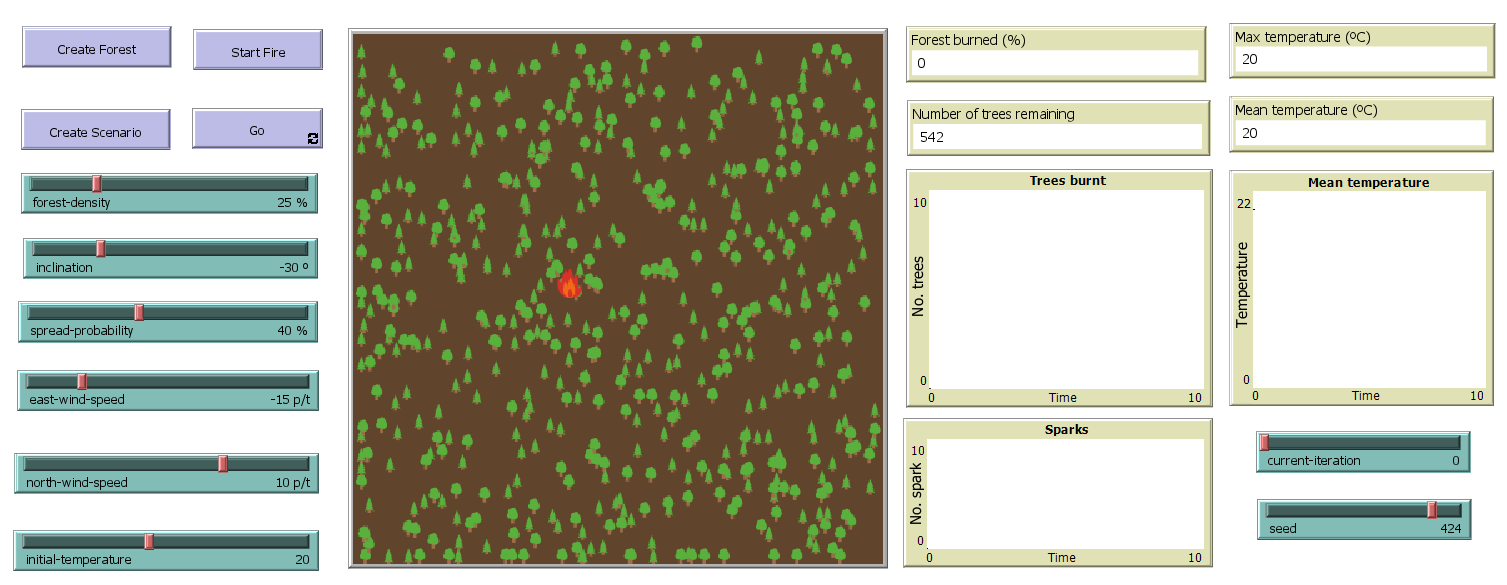
\includegraphics[width=\linewidth]{images/environment}
    \caption{Ambiente de simulação no NetLogo}
    \label{fig:environment}
\end{figure}

Além disso, a fim de poder retratar e avaliar diferentes cenários de incêndio, foi definido um conjunto de variáveis globais, com o recurso aos elementos gráficos do NetLogo, para representar quer propriedades da floresta em si, quer fatores ambientais que podem afetar a propagação do fogo.
Entre outros, o modelo prevê os seguintes parâmetros:

\begin{itemize}
    \item \texttt{forest-density} - a densidade da floresta, entre 0 e 100\%;
    \item \texttt{inclination} - a inclinação do terreno, entre \ang{-60} e \ang{60}, responsável pela altitude de cada célula;
    \item \texttt{east-wind-speed} - a velocidade do vento na direção leste (negativa se o vento soprar para o oeste), entre -25 e 25 p/t:
    \item \texttt{north-wind-speed} - a velocidade do vento na direção norte (negativa se o vento soprar para o sul), entre -25 e 25 p/t;
    \item \texttt{initial-temperature} - a temperatura inicial para cada célula do mundo, entre $\SI{0}{\degreeCelsius}$ e $\SI{45}{\degreeCelsius}$;
    \item \texttt{spark-frequency} - a frequência de ocorrência das fagulhas em ticks, por omissão, 150 ticks;
    \item \texttt{spread-probability} - a probabilidade de uma árvore ser incendiada pelo fogo, entre 0 e 100\%;
    \item \texttt{forest-seed} - a semente para o gerador de números aleatórios, entre 0 e 500;
    \item \texttt{current-run} - o número da \textit{run} atual de um dado cenário, entre 0 e 10;
    \item \texttt{iterations} - a lista de entradas contendo um \textit{snapshot} do modelo no final de cada \texttt{tick}.
\end{itemize}

Por fim, os patches também apresentam propriedades únicas, nomeadamente, \texttt{temperature} e \texttt{altitude}, que representam, respetivamente, a temperatura em cada célula à medida que o incêndio se propaga, e a altitude determinada pela inclinação do terreno.


\section{Algoritmo}\label{sec:algorithm}
O objetivo principal deste algoritmo é fornecer uma ferramenta eficiente para modelar e prever o comportamento dos incêndios florestais, permitindo a avaliação dos efeitos de diferentes cenários na propagação do fogo.
A simulação baseada em agentes é uma abordagem que considera a interação entre os elementos do ambiente e os agentes que nele atuam, permitindo a modelação de comportamentos complexos e dinâmicos.

O algoritmo descrito aqui considera fatores como topografia, vento, temperatura, a estrutura da comunidade vegetal e outros elementos relevantes para o comportamento do fogo.
A seguir, serão apresentados detalhes do funcionamento do algoritmo e como ele foi implementado para atender aos objetivos.

\SetKwFunction{calcAltitude}{calcAltitude}
\SetKwFunction{random}{random}
\SetKwFunction{plantTree}{plantTree}

\begin{algorithm}
    \caption{Criação da floresta (\texttt{createForest})}\label{alg:create_forest}
    $sparkFrequency \gets 150$\;
    $seed \gets forestSeed$\;
    \For{$patch \in patches$}{
        $altitude \gets \calcAltitude{pxcor}$\;
        $temperature \gets initialTemperature$\;
        \If{\random{$0, 100$} $<$ forestDensity}{
            \plantTree{pxcor, pycor}\;
        }
    }
\end{algorithm}

Em Alg.~\ref{alg:create_forest}, encontra-se detalhado o processo de população da floresta.
Este começa por definir a frequência, em ticks, de criação de fagulhas, seguido da atribuição da \textit{seed} responsável pela distribuição de árvores, bem como pela criação do fogo.
A cada célula é atribuída uma altitude dependente da sua posição, bem como uma temperatura inicial escolhida pelo utilizador.
Também, segundo a densidade da floresta, são plantadas árvores nos diferentes patches.

\SetKwFunction{ignite}{ignite}
\SetKwFunction{saveConfig}{saveConfig}
\SetKwFunction{anyTreesBurning}{anyTreesBurning}
\SetKwFunction{saveIteration}{saveIteration}
\SetKwFunction{saveIterations}{saveIterations}
\SetKwFunction{fire}{fire}

\begin{algorithm}
    \caption{Criação do fogo inicial (\texttt{startFire})}\label{alg:start_fire}
    $patch \gets \random(patches)$\;
    \ignite{patch}\;
    \saveConfig{}\;
    $seed \gets \random{seeds}$\;
    \While{\anyTreesBurning{}}{
        \saveIteration{}\;
        \fire{}\;
    }
    \saveIterations{}\;
\end{algorithm}

Com a floresta plantada, resta criar o fogo inicial, tal como se pode ver em Alg.~\ref{alg:start_fire}.
Começa-se por escolher aleatoriamente um ‘patch’, no qual é criada a primeira chama.
A seguir, são salvas as configurações do cenário em ficheiro YAML, e reiniciada a semente.
O modelo entra num ciclo condicional, responsável por salvar o estado do modelo em cada iteração e de propagar o incêndio.
Após o fim do ciclo, são guardados em ficheiro CSV os resultados das iterações.

\SetKwFunction{spreadFire}{spreadFire}
\SetKwFunction{canSpark}{canSpark}
\SetKwFunction{createSpark}{createSpark}
\SetKwFunction{forward}{forward}
\SetKwFunction{fadeEmbers}{fadeEmbers}
\SetKwFunction{tick}{tick}
\SetKwFunction{create}{create}

\begin{algorithm}
    \caption{Evolução do incêndio (\texttt{fire})}\label{alg:fire}
    \EndFor
    \For{$tree \in trees$}{
        \If{isBurning}{
            \If{$color < ``yellow"$}{
                \spreadFire{neighbors, altitude}\;
            }
            \If{$color < ``brown"$}{
                \If{$\random{0, 1} < sparkProbability$ \textbf{and} $ticksSinceSpark > sparkFrequency$}{
                    \create{spark}\;
                    $ticksSinceSpark \gets 0$\;
                }
                \Else{
                    $ticksSinceSpark \gets ticksSinceSpark + 1$\;
                }
            }
        }
    }
    \For{$spark \in sparks$}{
        \If{$position \neq finalPosition$}{
            \forward{$0.1$}\;
        }
        \Else{
            \ignite{patch-here}\;
        }
    }
    \fadeEmbers{}\;
    \tick{}\;
\end{algorithm}

O Algoritmo~\ref{alg:fire} representa o algoritmo responsável pela evolução do incêndio ao longo da execução do modelo.
Em cada tick, as árvores a arder espalham o fogo para as células vizinhas e geram fagulhas, segundo uma certa probabilidade, consoante a cor das suas folhas - esta representa o estado da árvore, mais ou menos queimada.
Já as fagulhas movem-se em direção à sua posição final, na qual incendeiam as árvores presentes.
Por fim, o estado de queima das árvores é atualizado com o procedimento \texttt{fadeEmbers}, responsável por alterar as propriedades da árvore, em particular a sua cor.

\begin{algorithm}
    \caption{Ignição do fogo (\texttt{ignite})}\label{alg:ignite}
    \create{fire}\;
    \For{$tree \in trees{-}here$}{
        \If{\textbf{not} ($isBurning$ \textbf{and} $isBurnt$)}{
            $isBurning \gets true$\;
        }
    }
\end{algorithm}

Para incendiar as árvores, recorremos ao procedimento \texttt{ignite}, definido em Alg.~\ref{alg:ignite}.
Este algoritmo é responsável por criar um agente \textit{fire} na célula atual, bem como de incendiar quaisquer árvores que não estejam a arder na mesma.

\SetKwFunction{towards}{towards}
\SetKwFunction{meanTemperature}{meanTemperature}

\begin{algorithm}
    \caption{Propagação do fogo (\texttt{spreadFire})}\label{alg:spread_fire}
    \KwIn{fireAltitude}
    $probability \gets spreadProbability$\;
    $direction \gets \towards{this}$\;
    \Switch{direction}{
        \Case{\ang{0}}{
            $probability \gets probability - northWindSpeed$\;
        }
        \Case{\ang{90}}{
            $probability \gets probability - eastWindSpeed$\;
        }
        \Case{\ang{180}}{
            $probability \gets probability + northWindSpeed$\;
        }
        \Case{\ang{270}}{
            $probability \gets probability + eastWindSpeed$\;
        }
    }
    $meanTemp \gets \meanTemperature{neighbors}$\;
    $probability \gets probability + \ln^2{(meanTemp + 1)}$\;
    \If{$fireAltitude > altitude$}{
        $probability \gets probability\cdot\left(1+|\tan\left(\frac{inclination}{3}\right)|\right)$\;
    }
    \If{\random{$0, 100$} $<$ probability}{
        \ignite{patch-here}\;
    }
\end{algorithm}

Por fim, temos o algoritmo responsável pela propagação do fogo em si, retratado em Alg.~\ref{alg:spread_fire}.
Começa-se por determinar a direção do fogo em relação à célula atual, e por inicializar a probabilidade de propagação com o valor definido pelo utilizador no início do programa.
A seguir, consoante a direção do vento, ajusta-se adequadamente esta, tal que o mesmo possa contribuir, positiva ou negativamente para essa propagação.
Segue-se o cálculo da temperatura média nas células vizinhas, sendo igualmente usada para modificar novamente a propriedade (quanto mais quente estiver o ambiente em redor, melhor se propaga o fogo).
Por fim, e porque o fogo tende a subir, quando enfrenta terrenos íngremes, a probabilidade é alterada uma última vez para refletir a inclinação do terreno.
Termina-se por incendiar a célula presente, segundo o valor final da probabilidade de propagação.

Todos os detalhes da implementação do modelo de simulação em NetLogo, bem como do módulo desenvolvido em Python para o processamento dos resultados, podem ser consultados no Apêndice~\ref{ch:appendix}.

